\section{Version 0.5}
In the fifth version the goal was to learn if it would be beneficial for the user to have another possibility to find books other that scanning the barcode of a book. Indications received from the customer and other users suggest the need of this functionality, and it was therefore selected as the assumption of this version. 
\subsection{Assumptions and questions}
The assumptions to be confirmed in this iteration was “Users want to be able to search for book by text”.

Questions used to verify this assumption:
\begin{enumerate}
    \item How are the users used to search in applications?
    \item On what type of information do the users want to search?
    \item What are the users interested in being returned from the search?
\end{enumerate}

\subsection{Planning and design}
Defining how to get answers to these questions was the first part of planning the version. Fortunately the indication that this was a desired feature had already been received from the customer representative which meant that the team could start directly with the design of the new feature in the applications. 

In the customer meeting held the day before this version, the customer representative had stated that both search and user validation was needed for the application to be a real \gls{MVP} that he could distribute to the employees at Netlight. Because the search functionality is a feature concerning the mobile applications, and the only support needed from \gls{backend} (filter on owners) was already implemented the \gls{backend} team would work on creating support for user validation (0.6) during this iteration.

To learn the answers to the first question, the team analyzed how some regularly used application like Facebook, Google Play for the Android users and AppStore and iBooks for the iOS users have implemented search functionality. In iOS the search is placed in the tab bar (bottom) shown in figure \ref{fig:ios-search-design}, while it is placed in the action bar (top) in the Android application.
\begin{figure}
\centering
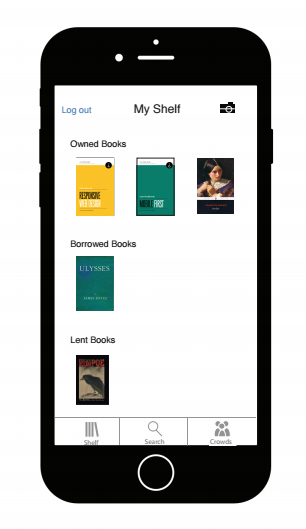
\includegraphics[height=7cm]{figs/v05/ios-search-design.png}
\caption{iOS design of search button}
\label{fig:ios-search-design}
\end{figure}


On the note of layout it was decided to renew the Android design during this version. Following the Android design principles, a new layout was defined. \cite{android-design} A color palette shown in figure \ref{fig:color-palette} selected from Google’s material design color palettes was selected for the application. In addition, the design team studied the design principles and other android applications, and concluded on a design illustrated from the shelf view in figure \ref{fig:android-design}

\begin{figure}
\centering
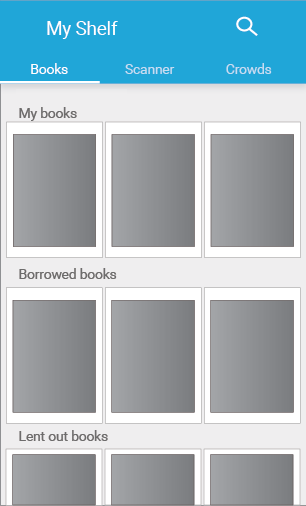
\includegraphics[height=6cm]{figs/v05/android-search-design.png}
\caption{The new Android color design with search button}
\label{fig:android-design}
\end{figure}

\begin{figure}
\centering
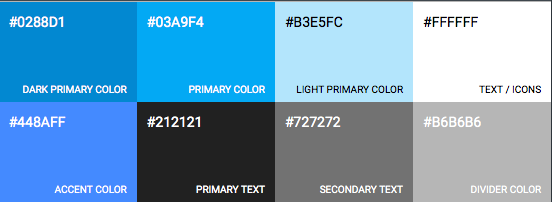
\includegraphics[height=4cm]{figs/v05/color-palette.png}
\caption{The color palette selected for the application}
\label{fig:color-palette}
\end{figure}

Question two and three was intended to be answered by the measurement of use in the application. In reference to the second question, the team decided that the users could search with any text they wanted, which would then search in Google Books and return that result. The team could then analyze what is searched using Mixpanel. This way if there are indications that the users do not get the results they want, for example if the same book is searched in different manners (author, title, ISBN) and only one of them returns a good result it might be preferable to let the users filter the search to what they are using to search.

The final question of what the users are interested in being returned from the search refers in addition to the design, to if they are interested in seeing all books, or just book owned by people in their groups. In the team it was decided to make both options possible by giving the user a filtering selection where they can choose between those two options. The team will then analyze what filter was used the most and make that the initial return of the search.

When planning this version the team decided to no longer use the term “Crowd” in the application, and instead use “Group” to describe the collections of users. This was decided in collaboration with the customer representative, and was discussed because the team had observed that some of the test persons from the usability tests had trouble understanding the meaning of a crowd.

After the measuring methods had been selected, three user stories were selected as the requirements needed to function in version 0.5. These user stories are shown in section \ref{user-stories-v5}


\subsection{User stories}
\label{user-stories-v5}
These user stories were selected to describe the functionality of version 0.5.
\begin{enumerate}
  \item As a user I want to search for books using ISBN
  \item As a user I want to search for books using title
  \item As a user I want to search for books using author
\end{enumerate}


\subsection{Development}
The implementation is still going well, and the teamwork has been great. The development for the different sub teams for this version is described in this section.
\subsubsection{Android}
\begin{description}
    \item[Features] \hfill\\
In version 0.5 the ability to search for books using text was implemented. The new search functionality allowed the user to choose between two different kinds of search, a local search in the user's groups and a search in the Google Books library. The search was implemented by adding a search button in the top right of the application's screen. When the user clicked on this button, a text field appeared next to the button, allowing the user to type in a search query. When the user confirmed the search query, it would search through groups the user was a member of in the realm database, and return a list of books that matched the search query. If the "search online"-button was clicked the application would search in the Google Books library.

Another new feature in this version was the possibility to view all the books a specific user is owning and all the books contained in a group. In earlier version of the application it was only possible to see if users had the book you were trying to borrow, not all the other books the user owned.

In the earlier version each book has been displayed as a different object, but in version 0.5 when choosing a book and viewing its information, information for all instances of the book was shown. This means that if a user had two copies of the same book and both were lent out, both renters would be shown in the book information. 

    \item[Structure] \hfill\\
In figure \ref{fig:AndroidDesign-05} a new activity has been added to the previous structure from version 0.4. The activity \code{SearchResultAcitivy} is the activity that handles how the search results from the user's search query are viewed on the screen. This activity also starts the \code{ViewBookActivity} activity if the user chooses a book from the list of books matching the search query, allowing the user the perform actions such as borrow or add on the selected book.

\begin{figure}
\centering
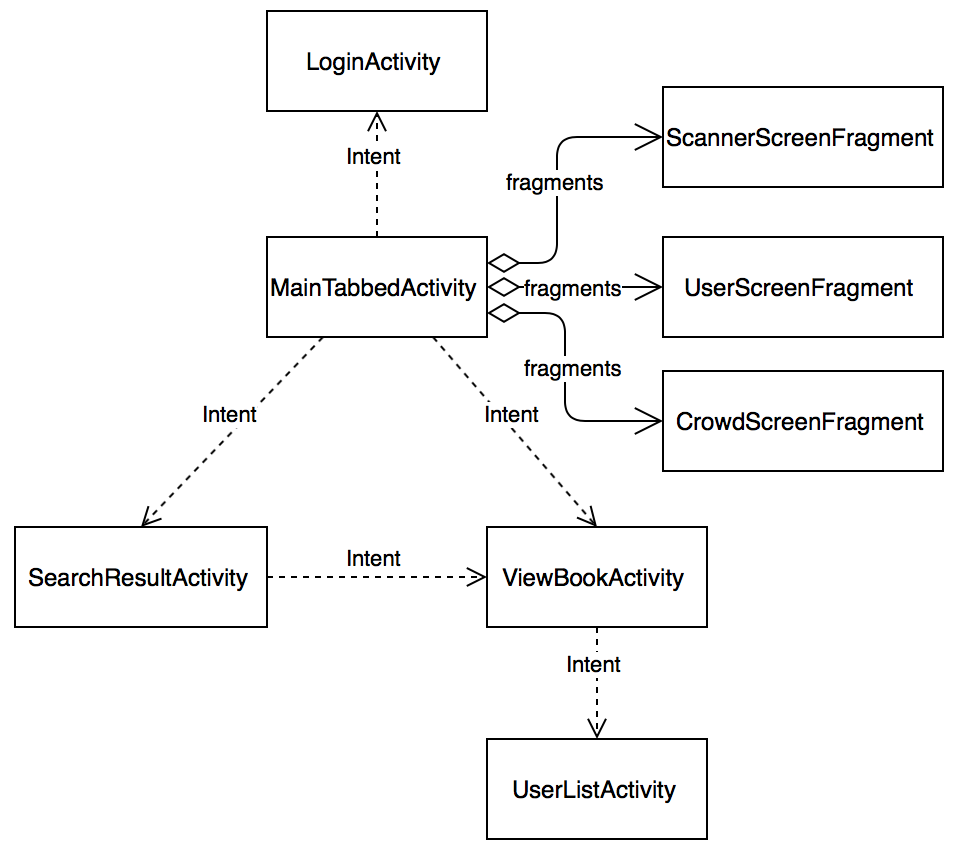
\includegraphics[height=7cm]{figs/v05/AndroidStructure-05.png}
\caption{Android version 0.5 structure}
\label{fig:AndroidDesign-05}
\end{figure}


    \item[Design] \hfill\\
Since the deadline for the project was approaching, the Android team decided to user more time on the design. They learned how it was possible to select a design and a set of color that should be used throughout the entire application. This means that if the team should decide to change the theme or color later they only need to do changes in one file. The team then used this design file to try to make the design follow the colors decided for the application. In figure \ref{fig:AndroidBookView05} it is possible to see how to book view have changed in this version (figure \ref{fig:androidcompare05}) from version 0.2 (figure \ref{fig:androidcompare02}).

\begin{figure}
\centering
\begin{subfigure}{.5\textwidth}
  \centering
  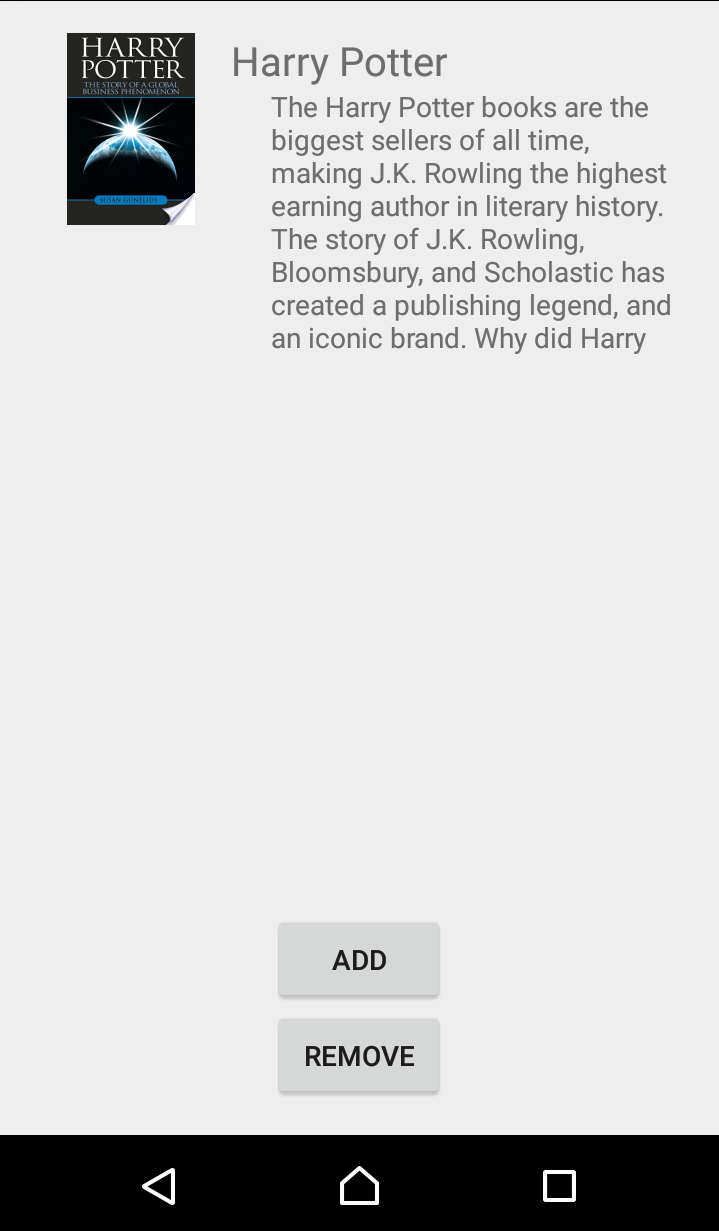
\includegraphics[width=.4\textwidth]{figs/v02/bookView02.png}
  \caption{Version 0.2}
  \label{fig:androidcompare02}
\end{subfigure}%
\begin{subfigure}{.5\textwidth}
  \centering
  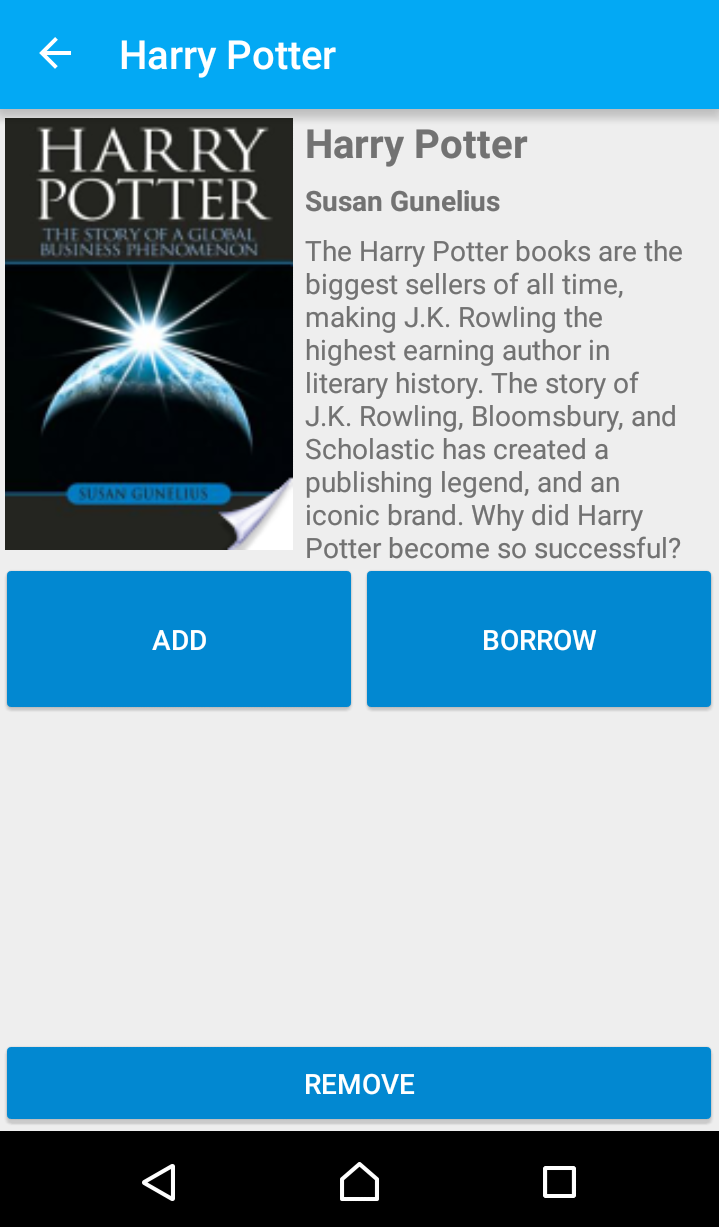
\includegraphics[width=.4\textwidth]{figs/v05/bookView05.png}
  \caption{Version 0.5}
  \label{fig:androidcompare05}
\end{subfigure}
\caption{Design changes from version 0.2 to version 0.5}
\label{fig:AndroidBookView05}
\end{figure}


    \item[User feedback] \hfill\\
In this version the team wanted to know if the users primary used search for searching in available books in the user's groups, or if the users used search to find books not already in the applications database to add these to their own shelf. To receive this feedback the event SwitchedFilter was added to Mixpanel, as shown in Table \ref{tab:mixpanel_table}. This allowed the team to track each time a user changed between local search and search in Google Books. 
\end{description}

\subsubsection{iOS}
\begin{description}
    \item[Features] \hfill\\
The iOS team spent this iteration implementing the new search feature, as requested by the customer. This was done sending a request with the users query to the Google Books API, and displaying the results as the user types. In an attempt to avoid the API's number of requests limitations, the requests were sent only after the query had been unchanged for at least 0.7 seconds. In order to filter the results to show only books in the users groups, a segmented controller was added to control the filter state. When the user selected the groups filter, a set of all available \gls{ISBN}s was compiled and used to filter the results from Google.

The shelf was also updated. It no longer show all the users unique books, but rather all the book titles the users owns. 

    \item[Design] \hfill\\
The team decided that moving the search feature in a dedicated view on the tab bar was the best approach for iOS. The existing scanner view was merged with the new search view in order to keep the tab bar clean and easy to use. To activate the scanner, the user had to navigate to the search view and press a camera button in the top, left corner. Search results were displayed as a list with the cover image and title of the book.

The scanner view was also improved with a rectangle showing the user where to position the barcode, and a new button which allows the user to activate or reactivate the device's torch for improved scanning in low light conditions.

\begin{figure}
\centering
\begin{subfigure}{.5\textwidth}
  \centering
  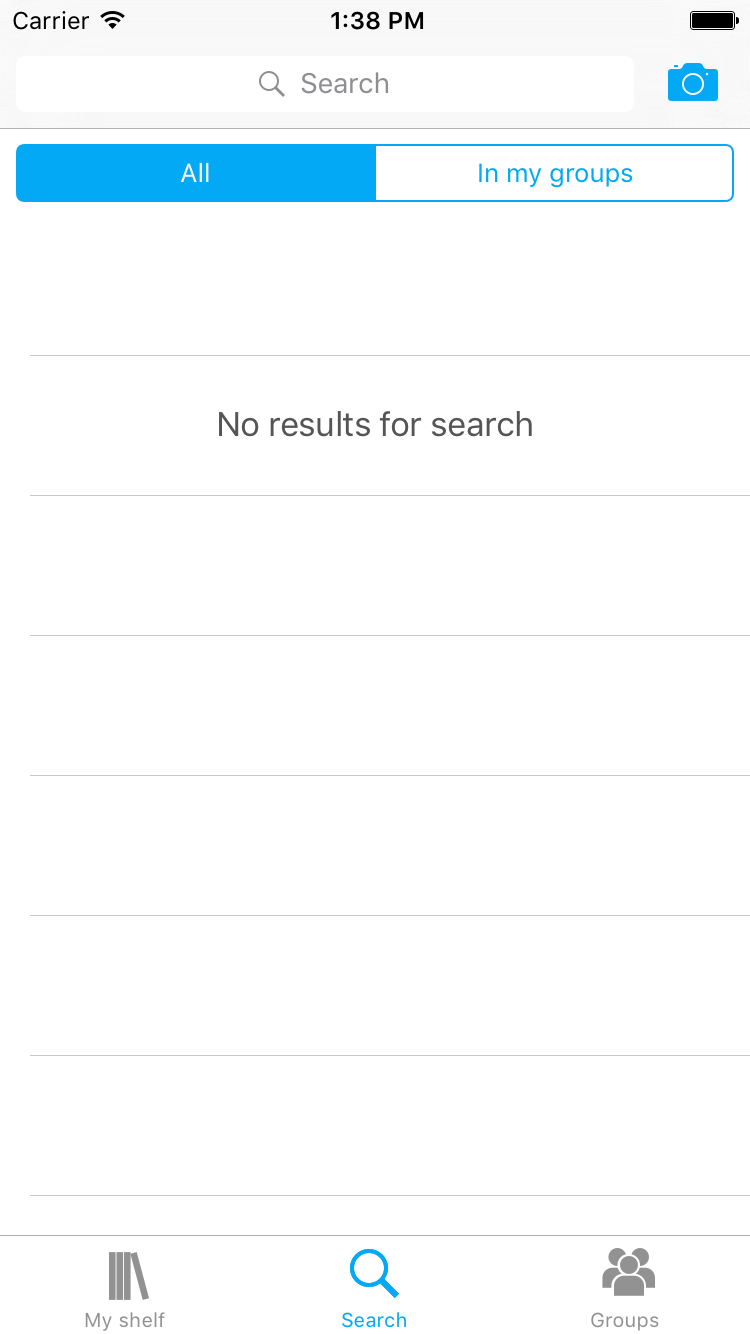
\includegraphics[width=.4\textwidth]{figs/v05/ios-search-view.png}
  \caption{Search empty view}
  \label{fig:ios-search-view-empty-5}
\end{subfigure}%
\begin{subfigure}{.5\textwidth}
  \centering
  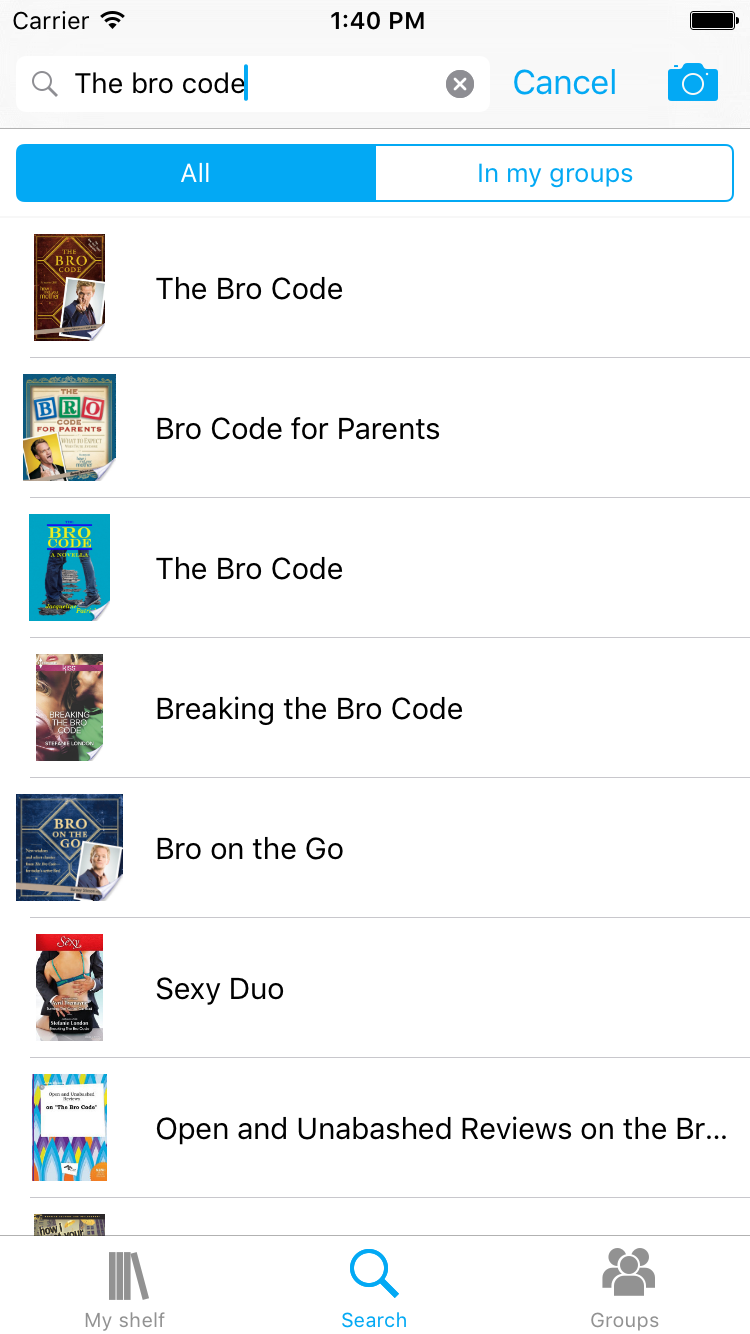
\includegraphics[width=.4\textwidth]{figs/v05/ios-search-results.png}
  \caption{Search view with results}
  \label{fig:ios-search-view-results-5}
\end{subfigure}
\caption{iOS search view design in version 0.5}
\label{fig:ios-search-view-5}
\end{figure}

\begin{figure}
\centering
\begin{subfigure}{.5\textwidth}
  \centering
  
\includegraphics[width=.4\textwidth]{figs/v02/ios-scanner-view.png}
  \caption{Version 0.2}
  \label{fig:ios-scanner-view-2}
\end{subfigure}%
\begin{subfigure}{.5\textwidth}
  \centering
  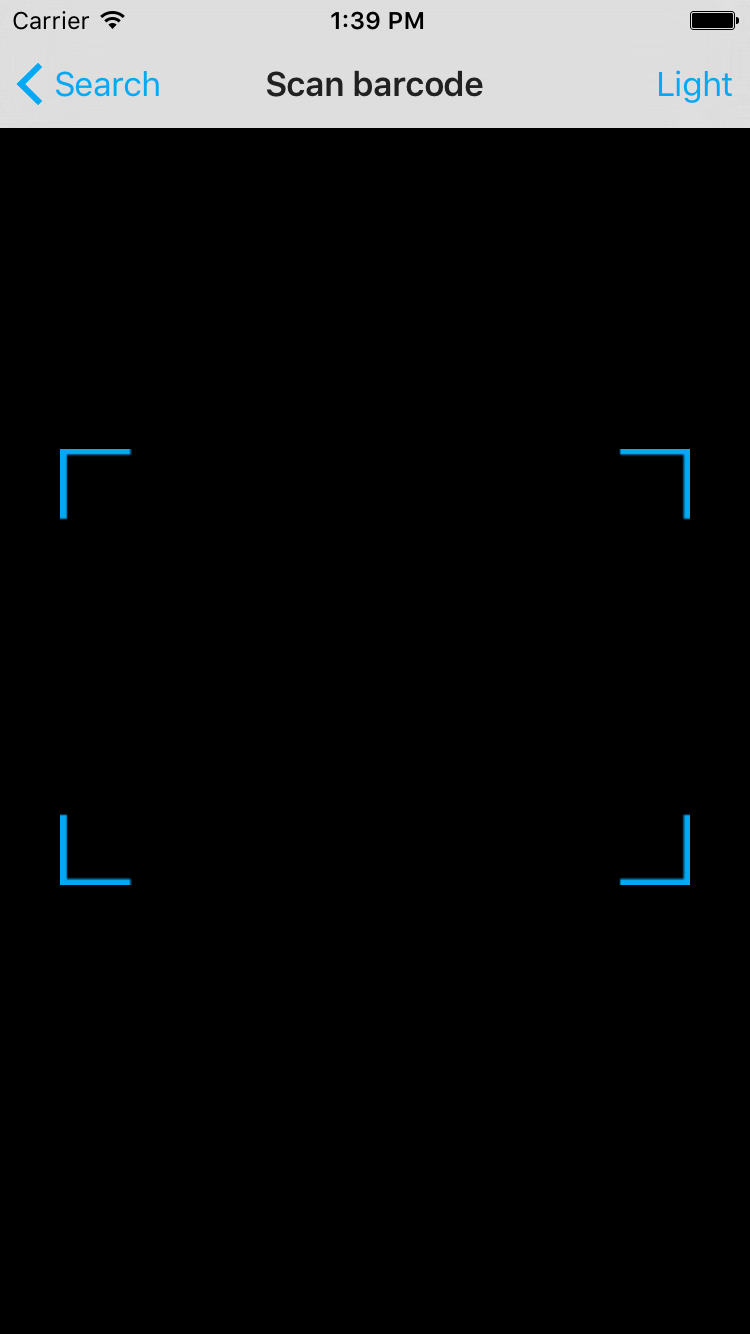
\includegraphics[width=.4\textwidth]{figs/v05/ios-scanner-view.png}
  \caption{Version 0.5}
  \label{fig:ios-scanner-view-results-5}
\end{subfigure}
\caption{Comparison of the old and new scanner design}
\label{fig:ios-scanner-view-comparison-5}
\end{figure}


    \item[Feedback] \hfill\\
The integration of Mixpanel from version 0.5 was extended to also include reporting the users search activity. This would allow the team to monitor how the new features were used.
\end{description}

\subsubsection{Backend}
For this iteration the \gls{backend} team was given the task of developing a full user service, as well as the possibility for the system to send e-mails, retrieve lost passwords and invite friends. In addition, the user stories from this iteration as well as the earlier ones, indicated that the team would need to develop a way for the users to authorize themselves, so that not all users could do all operations. Because all this had to be one huge update of the \gls{API}, the team decided to move the release of these features to version 0.6. See section \ref{v06-backend}.


\subsection{Feedback}
In answering the questions to confirm the assumption of this version the success was not satisfactory. The application was released containing the Mixpanel tracking to measure the use of both search and what result the users wanted, but there was not enough user data after version 0.5 was released to be able to say that the assumption was correct. On the other hand it did not imply that it was not correct either. Due to this, the feature was kept, but not improved until more feedback was received.

Even though the application received only a small amount of feedback, the customer representative had stated that both search and user validation was desired as mentioned in the planning section. Therefore, despite the lack of feedback from other users, the team could continue with implementing version 0.6.

\subsection{Version progress}
As shown in figure \ref{fig:version-progress-5} this version started on a Thursday, and the team did get to real work before the weekend was over. After that the progress was nice and steady, of course there was some differs in the number of tasks completed each day, but, this is because some of the tasks took longer to complete.

During this version the team really felt they had started to get a hang of the technical part of the project. The version was completed within the time limit, which was not that long, and the team did not encounter any major problems during the implementation. The blog posts describing this version are found in figures \ref{fig:week-nine} and \ref{fig:week-ten}

The tasks completed during version 0.5 are found in appendix \ref{app:release-note-5} including the user stories that the tasks were based upon. 

\begin{figure}
\centering
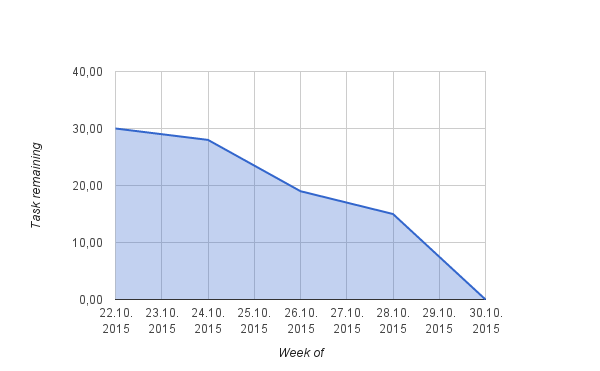
\includegraphics[height=10cm]{figs/v05/version-progress-5.png}
\caption{Task progress version 0.5}
\label{fig:version-progress-5}
\end{figure}

\begin{figure}
\centering
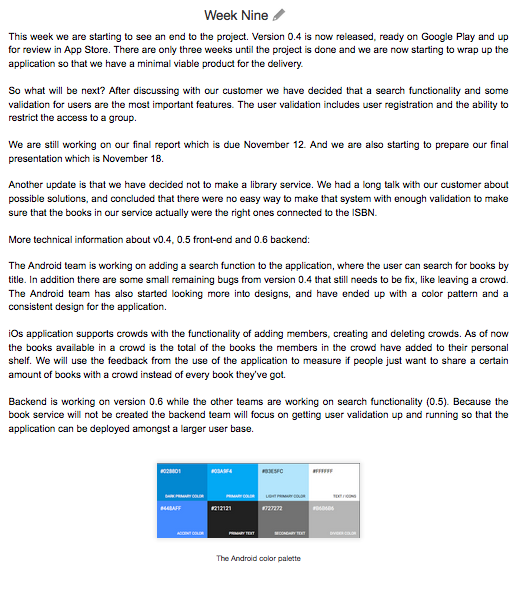
\includegraphics[height=17cm]{figs/v05/weekNine.png}
\caption{Blog post from week nine}
\label{fig:week-nine}
\end{figure}

\begin{figure}
\centering
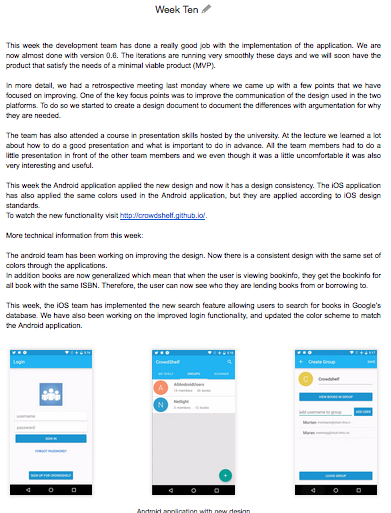
\includegraphics[height=20cm]{figs/v05/weekTen.png}
\caption{Blog post from week ten}
\label{fig:week-ten}
\end{figure}



\subsection{Review and retrospective}
Between version 0.5 and 0.6 the team did not have a customer meeting with the customer representative due to his job taking up most of that week. However, the customer representative had in the previous meeting told the team what was needed to create a \gls{MVP} and the team could therefore continue with the next version of the application.

After version 0.5 was complete the team had an internal retrospective meeting to discuss to progress and atmosphere of the project. The whiteboard with the opinions is shown in figure \ref{fig:retrospective-5}.
\begin{figure}
\centering
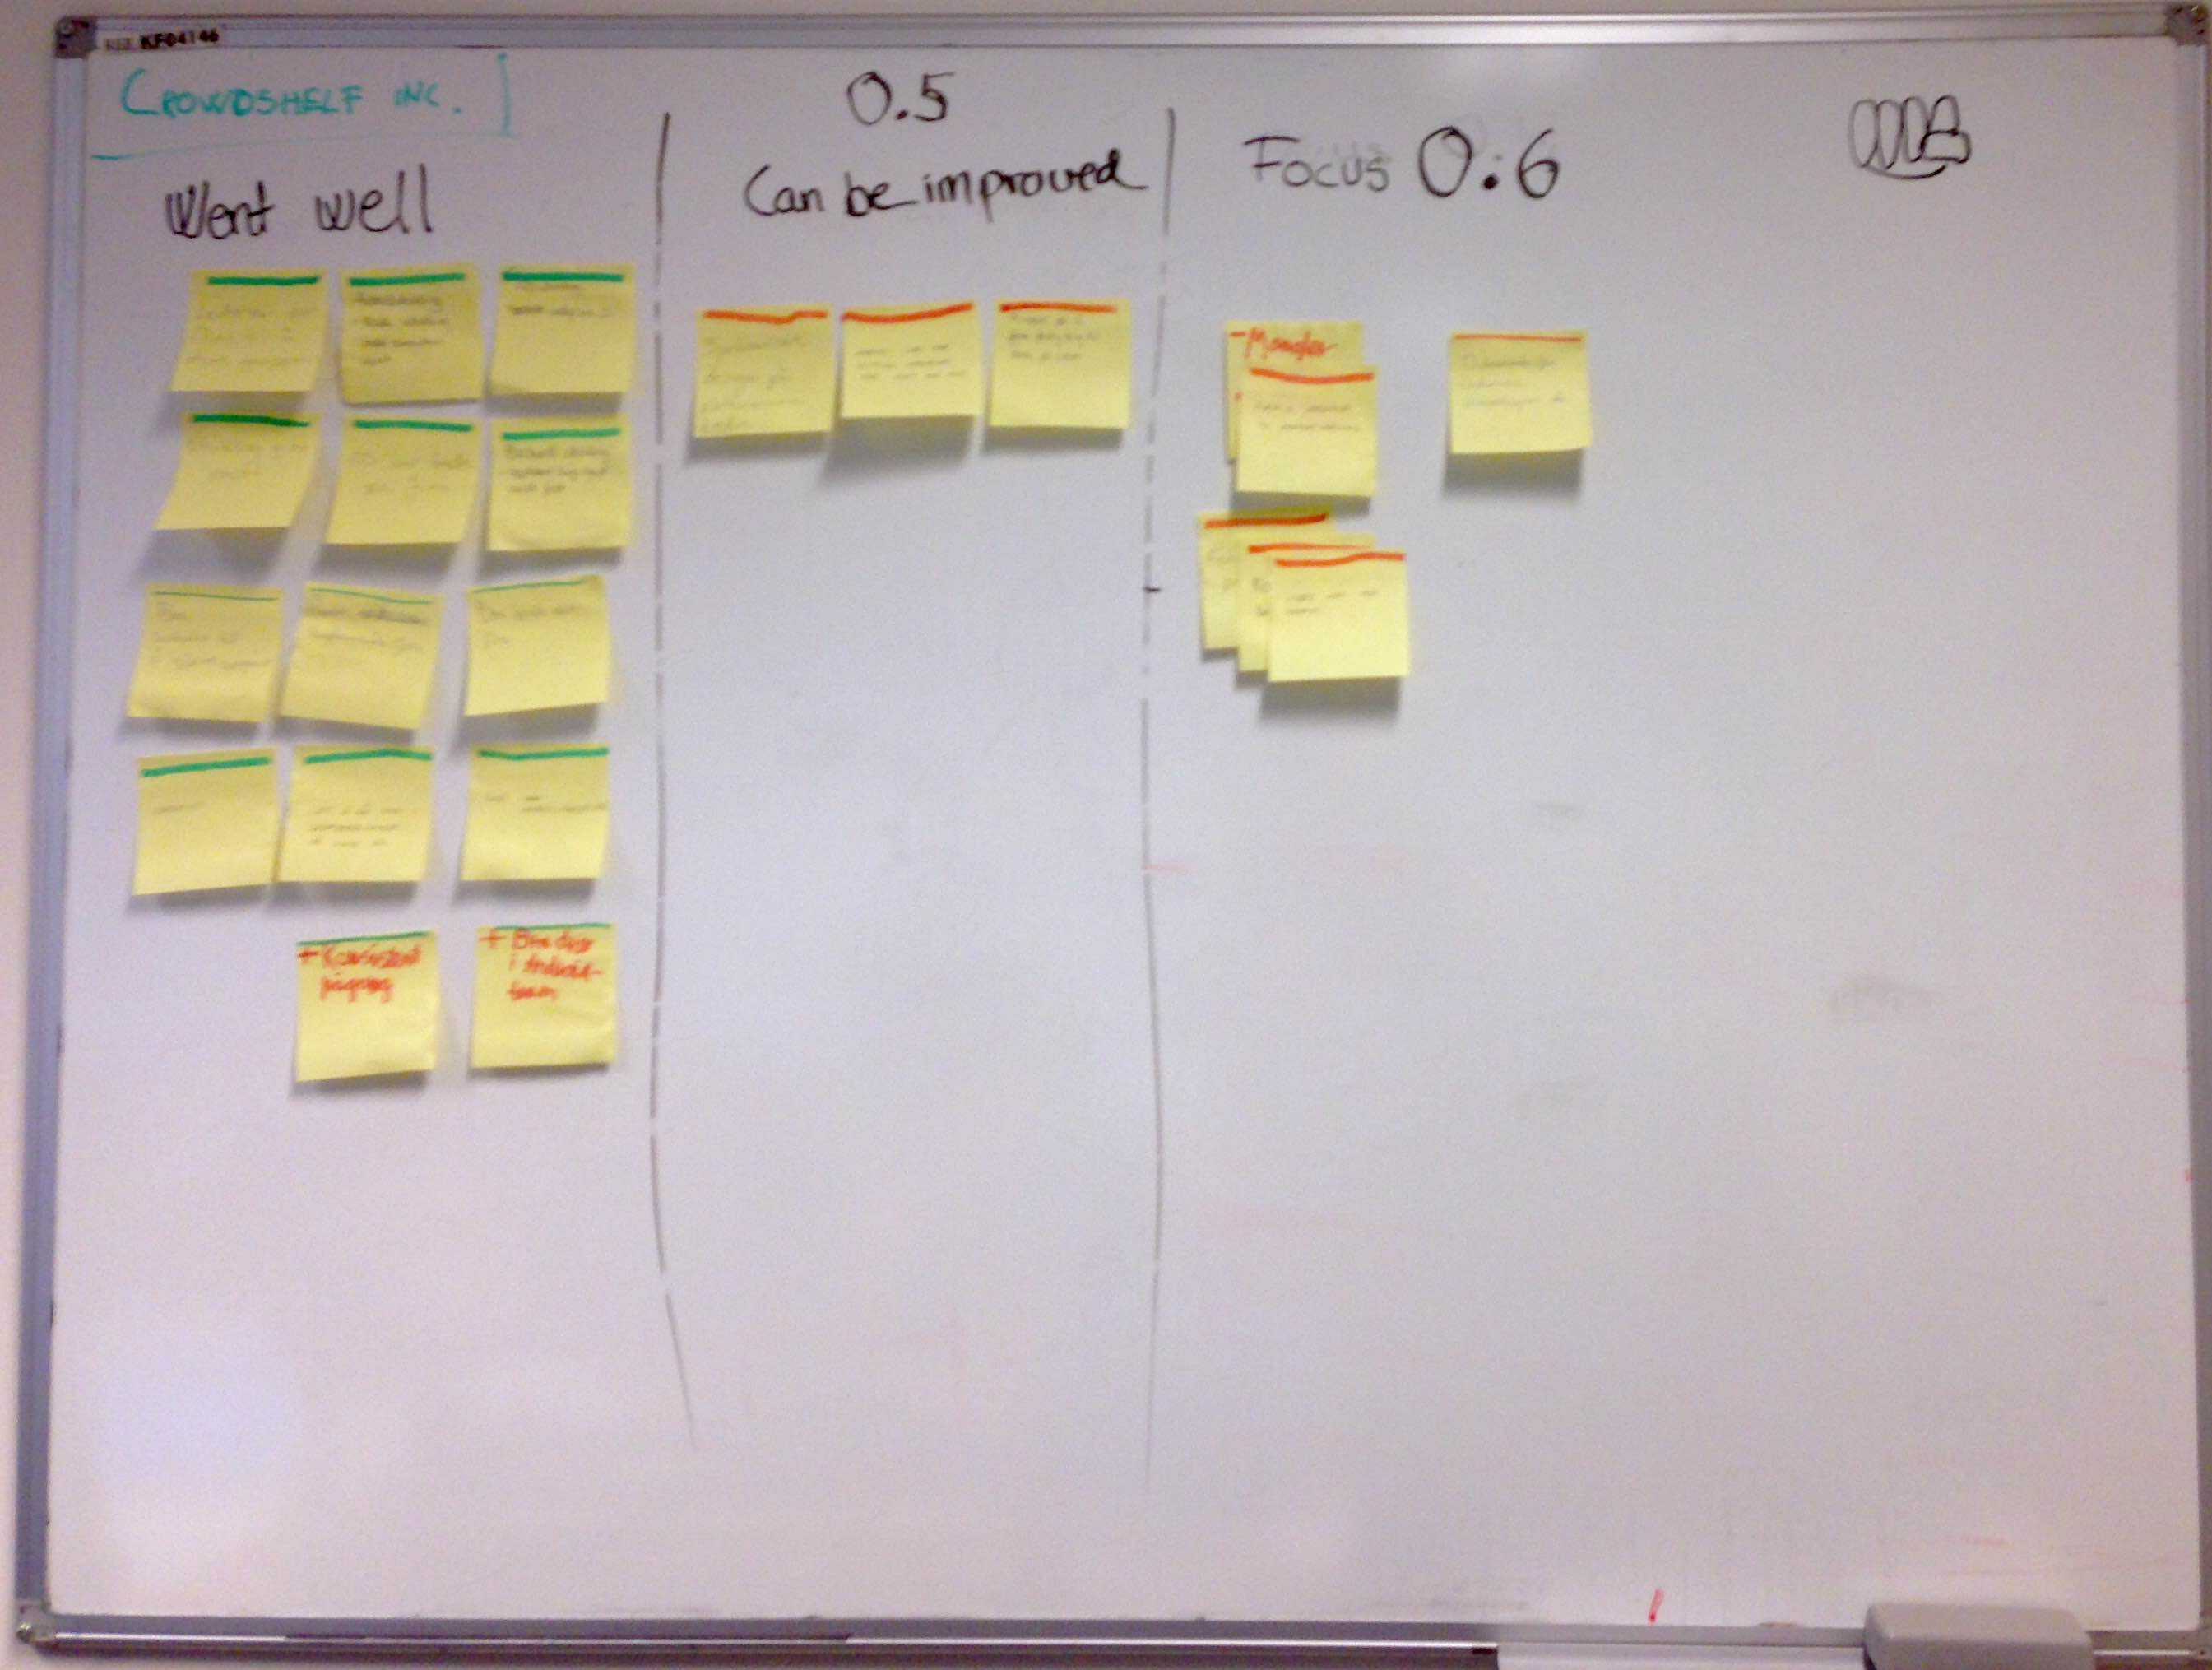
\includegraphics[height=10cm]{figs/v05/retrospective-5.JPG}
\caption{The whiteboard after the retrospective meeting of version 0.5}
\label{fig:retrospective-5}
\end{figure}

In this meeting there was a lot of positive feedback from the group. Some key points that went well this version was the smooth implementation of the product and especially the Android development that in earlier versions has taken a lot more time. Other than that there were mentions of good communication, quick response time, and a lot of initiative.

The improvement list has been shortened a lot since the first group retrospective meeting, but there are still some point to get better. First it is the synchronization of design on the two platforms which was mentioned at the last retrospective as well. The team has started to work on that. Other point were focusing on the essential tasks, not all the possible improvements, and get better at moving completed tasks to the Done-column in JIRA. The two things that were noticed by most of the members was the lack of report writing and the continuous documentation of the software being made. These points were selected as focus for version 0.6


\subsection{Summary}
During this version the design of both mobile application was updated. Search functionality was implemented in the mobile applications while the backend team worked on supporting user validation in parallel with fixing bugs that the mobile developers found when implementing their functionality. 

After discussing with the customer representative the team will develop version 0.6 that support of user validation and the application will then be distributed to employees at Netlight. 